The LHC collides protons at a rate of 40 MHz, producing an extraordinarily large amount of data (\~ 1.5 MB per event). Unfortunately, it is not feasible for ATLAS to record every single event that occurs because it would require storage capabilities that nowhere on Earth could provide. Instead, ATLAS employs a triggering system that reduces the event rate to 75 kHz by focusing only on events that could be considered interesting\@. The trigger system is divided into two levels: the Level-1 (L1) trigger and the High-Level Trigger (HLT)\@.

The L1 trigger is the first stage of the ATLAS trigger system and is entirely hardware based. It relies on FPGAs running custom algorithms to rapidly process detector data. At the center of the L1 trigger is the Central Trigger Processor which is fed signals from the Level-1 calorimeter (L1Calo) trigger and Level-1 muon (L1Muon) trigger.

The L1Calo trigger system is responsible for using calorimeter information to identify high energy photons, leptons, jets and the total \met{}. It is composed of three main components: the PreProcessor (PP), the Cluster Processor (CP), and the Jet/Energy Processor (JEP)\@. When the L1Calo trigger is activated, the TT sends a signal to a receiver system where the signal is amplified. The signals are then passed to the PP which digitizes the signals at the LHC bunch crossing rate. Additionally, the PP determines the \met{} and associated bunch crossing. These results are passed in parallel to the CP and JEP systems. The CP applies a clustering algorithm to count and identify electrons/photons and taus/hadrons that pass a predetermined threshold. JEP performs a similar function for jets. It also is responsible for calculating the \met{} and \met{} significance for each event. These results are then passed to the CTP\@. The L1Muon trigger system is responsible for determining the number of coincidence hits that each trigger station has within a certain window depending on a predetermined \pt{} threshold. Muons have six different thresholds, three correspond to low a \pt{} trigger within the range 6--9 GeV, and three for a high-\pt{} trigger, corresponding to 9--35 GeV. The trigger signals from the end-caps and barrel are combined into one set of six threshold multiplicities for each bunch-crossing. These signals are passed into the Muon CTP interface MUCTPI before being passed into the CTP.\@.

The CTP combines information passed to it from both the L1Calo and L1Muon trigger systems to make a decision on an event. A schematic of the trigger processing chain can be seen in Figure~\ref{fig:atlas_trigger_chain}.

\begin{figure}
    \centering
    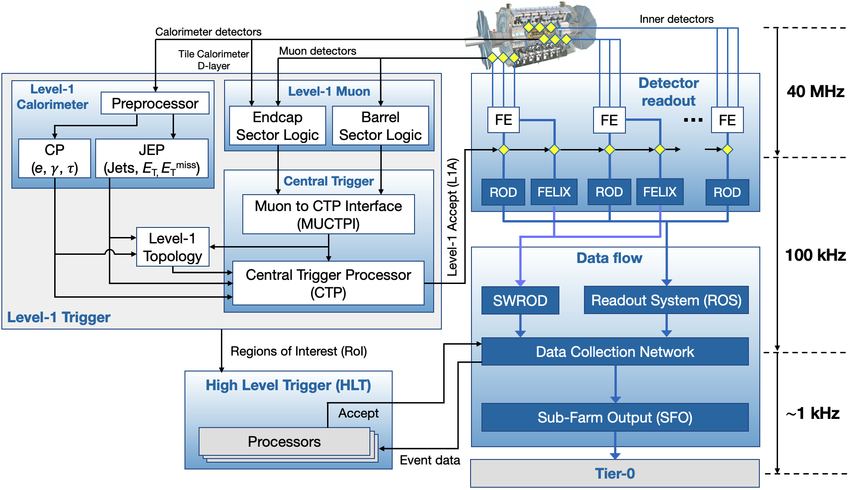
\includegraphics[width=0.8\textwidth]{figures/atlas/atlas_trigger_system.png}
\caption{A schematic showing the data flow in the trigger chain. Data is read out to both the L1Calo and L1Muon systems where logic is performed. These outputs from these triggering systems are then passed onto the CTP to determine if this event is worth a more in-depth analysis. Finally, the event information is passed onto the High Level Trigger where the final decision of whether the event is recorded or not is decided. Taken from~\cite{atlas_trigger_system}.}\label{fig:atlas_trigger_chain}
\end{figure}
